\section{Betriebssystem}
	Die mobilen Betriebssysteme iOS und Android sind die zum Stand dieser Arbeit
	meist genutzten weltweit. Im März 2015 hatte iOS in den USA einen
	Marktanteil von 36,5\%, während Android diesen mit 58,1\% angeführt hatte.
	Dagegen war der Marktanteil von iOS in Deutschland zeitgleich nahezu auf 18,3\%
	halbiert, während Android deutlich höhere 71,3\% besaß\cite{MobileOsStat}.
	\begin{figure}[h]
		\centering
		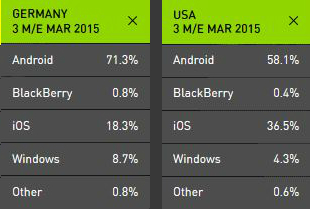
\includegraphics[width=0.5\linewidth]{ios/media/marketshare-cmp-201503.jpg}
		\caption{Marktanteil der mobilen Betriebssysteme
		\cite{MobileOsStat}}
		\label{fig:marcetshare}
	\end{figure}